% !TEX root = main_min_disc_dist.tex
\subsection{Double Integrator}
The doube integrator consists of two states $(x_1, x_2)$ , and  control $u \in [-u_{max}, u_{max}]$ with dynamics,
\begin{equation}
\begin{split}
\dot{x_1} & = x_2 \\
\dot{x_2} & = u 
\end{split}
\end{equation}
\noindent The state space is discretized into a $161 \times 161$ grid on the domain $[-1,5] \times [-5,5]$, and $u_{max}=2$.

The task is to keep the state trajectory inside the box $\K = [0,4] \times [-3,3]$, thus the target is taken to be its compliment $\T=\K^C$. For ease of exposition we define the \emph{safe set} $\Omega(\T) := \R(\T)^C$.

We first show, in Fig~\ref{fig:convergence} that different level curves of $Z$ over approximates~(bold line) and under approximates~(dotted lines) the analytic safe set~(shown in black) for two values of $\lambda = 0.1, 0.2$, with $\bar{\tau}=2$. As expected smaller values of $\lambda$, yield tighter approximations. 

To verify the convergence properties of the MDR formulation we initialize value iteration with the zero vector $\vec{0}\in \RR^{N_G}$ with $\lambda=0.1$. The error (in the infinity norm) between the converged solution and the one visualized in Fig~\ref{fig:convergence} is $0.000299$, suggesting convergence to the same fixed point. Under the MR setting value iteration fails to converge with this particular initialization.

\begin{figure}
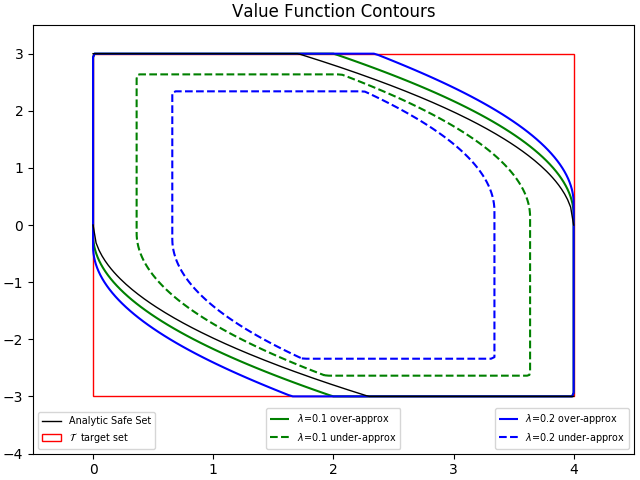
\includegraphics[scale=0.5]{convergence_difflambda.png}
\caption{The analytic safe set and target set $\mathcal{T}$ are shown in black (interior) and red (exterior), respectively. The over and under approximated $Z$ are shown in bold green and dotted green for $\lambda=0.1$; and bold blue and dotted blue line for $\lambda  = 0.2$ (all interior).}
\label{fig:convergence}
\end{figure}

We now compare value iteration and policy iteration with increasing number of discrete actions in Table~\ref{tab:v_vs_p}. In the table we see that the runtime of value iteration increases linearly with the increase in the number of actions, and policy iteration scales much better. The overall runtime favors value iteration, but it is important to note that the majority of the time in policy iteration is spent constructing $\Phi_{\pi_u}$, which is denoted by $T_{\Phi_{\pi_u}}$.\footnote{The data structure used to represent the interpolation is very efficient for sparse matrix multiplication, but is not ideal for indexing, which is necessary to create $\Phi_{\pi_u}$.} Excluding this cost, policy iteration becomes more attractive.

\begin{table}
\centering
\caption{Value Iteration vs Policy Iteration}
\label{tab:v_vs_p}
\begin{tabular}{|c| c| c| c|}
\hline
\# actions & VI & \multicolumn{2}{|c|}{Policy Iteration} \\ \cline{3-4}
 &  $T_{total} $ & $T_{total}$ & $T_{total} - T_{\Phi_{\pi_u}}$ \\ \hline
2 & 1.468  & 78.197  & 0.102 \\ \hline
50 &  8.753 &  302.456 & 1.007 \\ \hline
250 & 36.973 &  308.565 & 4.318 \\ \hline
500 & 65.305 &  326.280 & 9.760\\
\hline
\end{tabular}
\end{table}

Next, we look at a multigrid approach versus value iteration. For the multigrid approach we also need to run value iteration on a coarse grid, which we construct to have half the resolution per dimension of the nominal grid, e.g. if the nominal grid has $41^2$ nodes then the coarse grid has $21^2$ nodes. The results are shown in Table~\ref{tab:multigrid_di}. We first run value iteration with the standard initialization on both the coarse and fine grid. This produces the values in columns two and three. We then run value iteration on the fine grid initialized with the coarse solution (CS), which makes up column four. Column five (multigrid) is obtained by adding columns two and four. From the table it is clear that the multigrid approach outperforms value iteration, especially as the number of nodes increases.

\begin{table}
\centering
\caption{Double Integrator: Value iteration (VI) with Multigrid}
\label{tab:multigrid_di}
\begin{tabular}{|c| c| c| c| c| }
\hline
\# nodes & Coarse grid & Fine grid &  Fine grid with CS & Multigrid \\ \hline
$40^2$ & $0.012$ & $0.025$ & $0.019$ & $0.031$ \\ \hline
$80^2$ & $0.019$ & $0.116$ & $0.041$ & $0.060$\\ \hline
$160^2$ & $0.153$ & $1.110$ & $0.084$ & $0.237$\\ \hline
\end{tabular}
\end{table}

Lastly, denoting the current model as nominal model $M_n$, we construct two different models: a heavy model $M_h$ with $u_{max}=1.0$, and a light model $M_l$ with $u_{max}=4.0$. This can be interpreted as two systems that have different control authorities due to their different masses. The $M_n$ MDR value function will be less than that of model $M_l$, but greater than that of $M_h$. We compute the value functions for $M_l$ and $M_h$ both initialized with the default initialization, and with the solution for model $M_n$, which we refer to as a \emph{warm start} (WS). The results are shown in Table~\ref{tab:ws_di}.

\begin{table}
\centering
\caption{Double Integrator: Value Iteration (VI) with Warm Start (WS)}
\label{tab:ws_di}
\begin{tabular}{|c| c| c| c| c| c|}
\hline
\# nodes & $M_n$ & $M_l$ &  $M_l$ with WS & $M_h$ & $M_h$ with WS \\ \hline
$40^2$ & $0.029$ & $0.044$ & $0.041$ & $0.022$ & $0.014$\\ \hline
$80^2$ & $0.205$ & $.364$ & $0.273$ & $0.097$ & $0.095$\\ \hline
$160^2$ & $1.444$ & $2.727$ & $2.304$ & $1.257$ & $1.116$\\ \hline
\end{tabular}
\end{table}



